\section{Data}

We evaluate our models on the color dataset used in \citep{monroe-2017-colors}. This dataset was generated by playing reference games where the color descriptions were produced by human participants in the speaker role. On each round of the game, the speakers were presented with three color patches, one of which was selected to be the target color. The speakers were instructed to communicate this information to the listeners who were asked to click on one of the colors to complete the task \citep{monroe-2017-colors}.

\par
The dataset contains 49,025 examples in total and was split to train and test set with 46,994 and 2,031 examples respectively. Every dataset comprises examples containing three colors, one of them being the target color to be described and the other two being distractor colors. Every example belongs to one of three conditions: 1) \emph{close}, where all three colors are similar, 2) \emph{split}, where one of the colors is close to the target colors and 3) \emph{far}, where all three colors are far apart in the color space \citep{monroe-2017-colors}. Table \ref{table:colors} shows one example of each condition.

\begin{table}[ht]
\centering
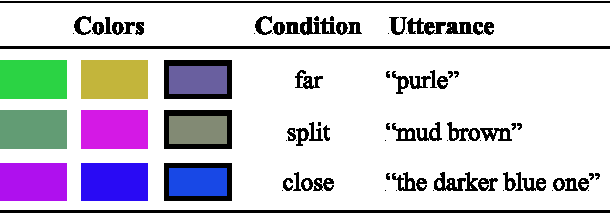
\includegraphics[width=\columnwidth]{assets/colors.pdf}
\caption[Colors]{Three color patches, represented using HLS values, are presented to the speaker. Each color patch set belongs to one of three conditions - far, split, close. The speakers describe the target color (marked with frame) to the listener (utterance).}
\label{table:colors}
\end{table}

\par
40.8\% of the \emph{train} dataset color descriptions use one word, 59.2\% use two or more with the majority being shorter than 14 words. All conditions are represented equally with 15,519 examples for the \emph{close}, 15,693 examples for the \emph{split} and 15,782 examples for the \emph{far} condition. The train dataset is further divided using 75/25 train-dev split while training.

\par
The \emph{test} dataset has a slightly different composition. 40.2\% of the color descriptions use one word, 54.6\% use two words and only 5.2\% use three or more words. The conditions are represented with 633 examples for the \emph{close}, 652 for the \emph{split} condition and 746 for the \emph{far} condition.